%%
%% This is file `sample-sigplan.tex',
%% generated with the docstrip utility.
%%
%% The original source files were:
%%
%% samples.dtx  (with options: `sigplan')
%% 
%% IMPORTANT NOTICE:
%% 
%% For the copyright see the source file.
%% 
%% Any modified versions of this file must be renamed
%% with new filenames distinct from sample-sigplan.tex.
%% 
%% For distribution of the original source see the terms
%% for copying and modification in the file samples.dtx.
%% 
%% This generated file may be distributed as long as the
%% original source files, as listed above, are part of the
%% same distribution. (The sources need not necessarily be
%% in the same archive or directory.)
%%
%%
%% Commands for TeXCount
%TC:macro \cite [option:text,text]
%TC:macro \citep [option:text,text]
%TC:macro \citet [option:text,text]
%TC:envir table 0 1
%TC:envir table* 0 1
%TC:envir tabular [ignore] word
%TC:envir displaymath 0 word
%TC:envir math 0 word
%TC:envir comment 0 0
%%
%%
%% The first command in your LaTeX source must be the \documentclass command.
\documentclass[sigplan,anonymous,review]{acmart}

%%
%% \BibTeX command to typeset BibTeX logo in the docs
\AtBeginDocument{%
  \providecommand\BibTeX{{%
    Bib\TeX}}}

%% Rights management information.  This information is sent to you
%% when you complete the rights form.  These commands have SAMPLE
%% values in them; it is your responsibility as an author to replace
%% the commands and values with those provided to you when you
%% complete the rights form.
\setcopyright{acmcopyright}
\copyrightyear{2018}
\acmYear{2018}
\acmDOI{XXXXXXX.XXXXXXX}

%% These commands are for a PROCEEDINGS abstract or paper.
\acmConference[Conference acronym 'XX]{Make sure to enter the correct
  conference title from your rights confirmation emai}{June 03--05,
  2018}{Woodstock, NY}
\acmPrice{15.00}
\acmISBN{978-1-4503-XXXX-X/18/06}


%%
%% Submission ID.
%% Use this when submitting an article to a sponsored event. You'll
%% receive a unique submission ID from the organizers
%% of the event, and this ID should be used as the parameter to this command.
%%\acmSubmissionID{123-A56-BU3}

%%
%% For managing citations, it is recommended to use bibliography
%% files in BibTeX format.
%%
%% You can then either use BibTeX with the ACM-Reference-Format style,
%% or BibLaTeX with the acmnumeric or acmauthoryear sytles, that include
%% support for advanced citation of software artefact from the
%% biblatex-software package, also separately available on CTAN.
%%
%% Look at the sample-*-biblatex.tex files for templates showcasing
%% the biblatex styles.
%%

%%
%% The majority of ACM publications use numbered citations and
%% references.  The command \citestyle{authoryear} switches to the
%% "author year" style.
%%
%% If you are preparing content for an event
%% sponsored by ACM SIGGRAPH, you must use the "author year" style of
%% citations and references.
%% Uncommenting
%% the next command will enable that style.
%%\citestyle{acmauthoryear}

%A set of custom commands that are used for my personal latex style
%Created: Feb 2020
%Updated: July 2020
\usepackage{listings}

\newcommand{\defn}[1]{\textbf{#1}} %definitions are bold
\newcommand{\jnote}[1]{\textcolor{blue}{Justin: #1\\}} %a note from Justin
\newcommand{\rnote}[1]{\textcolor{orange}{Ron: #1\\}} %a note from Ron
\newcommand{\pnote}[1]{\textcolor{purple}{Peyton: #1\\}} %a note from Peyton
\newcommand{\todo}[1]{\textcolor{red}{TODO: #1\\}} %a todo note

\definecolor{tangerine}{RGB}{245,166,35} %comments, primary color
\definecolor{blueSeaFoam}{RGB}{80,227,194}
\definecolor{liteGreen}{RGB}{184,233,134 }
\definecolor{royalBlue}{RGB}{74,144,226} %keywords
\definecolor{amaranth}{rgb}{0.9, 0.17, 0.31} %special keywords
\definecolor{lavender}{rgb}{0.71, 0.49, 0.86}

\lstdefinestyle{mystyle}{
    backgroundcolor=\color{white},   
    commentstyle=\color{tangerine},
    keywordstyle=\color{royalBlue},
    identifierstyle=\color{black},
    numberstyle=\tiny\color{gray},
    basicstyle=\ttfamily\footnotesize,
    breakatwhitespace=false,         
    breaklines=true,                 
    captionpos=b,                    
    keepspaces=true,                 
    numbers=left,                    
    numbersep=5pt,                  
    showspaces=false,                
    showstringspaces=false,
    showtabs=false,                  
    tabsize=2,
    frame=lines,
    %just for Chisel
    emph={Module, IO, Input, Output, UInt, Bool, Wire, Vec, before, after, extend, in, register, insert, apply, Pointcutter, AfterToken},
    emphstyle=\color{amaranth}
}

\lstset{style=mystyle}
\raggedbottom


%%
%% end of the preamble, start of the body of the document source.
\begin{document}

%%
%% The "title" command has an optional parameter,
%% allowing the author to define a "short title" to be used in page headers.
\title{Foam: Feature-Oriented Construction of Finite State Machines}

%%
%% The "author" command and its associated commands are used to define
%% the authors and their affiliations.
%% Of note is the shared affiliation of the first two authors, and the
%% "authornote" and "authornotemark" commands
%% used to denote shared contribution to the research.
\author{Ben Trovato}
\authornote{Both authors contributed equally to this research.}
\email{trovato@corporation.com}
\orcid{1234-5678-9012}
\author{G.K.M. Tobin}
\authornotemark[1]
\email{webmaster@marysville-ohio.com}
\affiliation{%
  \institution{Institute for Clarity in Documentation}
  \streetaddress{P.O. Box 1212}
  \city{Dublin}
  \state{Ohio}
  \country{USA}
  \postcode{43017-6221}
}

\author{Lars Th{\o}rv{\"a}ld}
\affiliation{%
  \institution{The Th{\o}rv{\"a}ld Group}
  \streetaddress{1 Th{\o}rv{\"a}ld Circle}
  \city{Hekla}
  \country{Iceland}}
\email{larst@affiliation.org}

\author{Valerie B\'eranger}
\affiliation{%
  \institution{Inria Paris-Rocquencourt}
  \city{Rocquencourt}
  \country{France}
}

\author{Aparna Patel}
\affiliation{%
 \institution{Rajiv Gandhi University}
 \streetaddress{Rono-Hills}
 \city{Doimukh}
 \state{Arunachal Pradesh}
 \country{India}}

\author{Huifen Chan}
\affiliation{%
  \institution{Tsinghua University}
  \streetaddress{30 Shuangqing Rd}
  \city{Haidian Qu}
  \state{Beijing Shi}
  \country{China}}

\author{Charles Palmer}
\affiliation{%
  \institution{Palmer Research Laboratories}
  \streetaddress{8600 Datapoint Drive}
  \city{San Antonio}
  \state{Texas}
  \country{USA}
  \postcode{78229}}
\email{cpalmer@prl.com}

\author{John Smith}
\affiliation{%
  \institution{The Th{\o}rv{\"a}ld Group}
  \streetaddress{1 Th{\o}rv{\"a}ld Circle}
  \city{Hekla}
  \country{Iceland}}
\email{jsmith@affiliation.org}

\author{Julius P. Kumquat}
\affiliation{%
  \institution{The Kumquat Consortium}
  \city{New York}
  \country{USA}}
\email{jpkumquat@consortium.net}

%%
%% By default, the full list of authors will be used in the page
%% headers. Often, this list is too long, and will overlap
%% other information printed in the page headers. This command allows
%% the author to define a more concise list
%% of authors' names for this purpose.
\renewcommand{\shortauthors}{Trovato et al.}

%%
%% The abstract is a short summary of the work to be presented in the
%% article.
\begin{abstract}
  Finite-State Machines are really cool.
\end{abstract}

%%
%% The code below is generated by the tool at http://dl.acm.org/ccs.cfm.
%% Please copy and paste the code instead of the example below.
%%
\begin{CCSXML}
<ccs2012>
<concept>
<concept_id>10011007.10011006.10011041.10011047</concept_id>
<concept_desc>Software and its engineering~Source code generation</concept_desc>
<concept_significance>500</concept_significance>
</concept>
<concept>
<concept_id>10010583.10010682.10010689</concept_id>
<concept_desc>Hardware~Hardware description languages and compilation</concept_desc>
<concept_significance>500</concept_significance>
</concept>
</ccs2012>
\end{CCSXML}

\ccsdesc[500]{Software and its engineering~Source code generation}
\ccsdesc[500]{Hardware~Hardware description languages and compilation}

%%
%% Keywords. The author(s) should pick words that accurately describe
%% the work being presented. Separate the keywords with commas.
\keywords{feature-oriented programming, finite state machines, generative programming, hardware generation}
%% A "teaser" image appears between the author and affiliation
%% information and the body of the document, and typically spans the
%% page.

%%
%% This command processes the author and affiliation and title
%% information and builds the first part of the formatted document.
\maketitle

\section{Introduction}

The advent of hardware-generation languages~\cite{hwgen} has promoted the adoption of techniques and abstractions by hardware designers that were previously available only to software systems and their designers.   Hardware-characterization languages such as VHDL~\cite{vhdl} and Verilog~\cite{verilog} describe the components and interconnections of hardware circuit elements, much like HTML describes the components and references of a web page.  While those languages provide some abstractions (such as arithmetic operations and restrictive macros), the paradigms and practices used widely in successful software engineering efforts are largely unavailable.

By contrast, hardware-generation approaches allow a designer to write a program, and the output of that program's execution is the hardware design.  The program can be authored using paradigms that promote efficient software construction, reuse, rigorous testing, and clarity of expression.  Our work in this paper builds on the hardware-generation language Chisel~\cite{chisel:book}, which is in turn built on Scala~\cite{scala-overview-tech-report}.   Chisel is essentially a Scala library that generates Verilog when a hardware design is executed.

A simple and recent example showing the advantages of hardware generation over characterization concerns an adder~\cite{Deters:adder}.   Using VHDL, a hardware designer can request that an adder circuit be optimized for either for delay (carry lookahead) or for area (carry propagate).   Using Chisel, an adder can be specified that combines both forms of carry computation, to meet a timing or area constraint while otherwise optimized in the other dimension.

Chisel has also proven itself robust in pedagogy and industry, serving as the basis for courses in digital logic~\cite{vlsicourse} and serving as a platform for describing RISC-V systems~\cite{chisel:riscv}.  Our long-term goal

In this paper, we consider a feature-oriented approach to generating hardware, specifically finite state machines.  A given feature can affect multiple regions of a finite state machine.  For example, the cache system  we consider in Section~\ref{sec:cache} could use write-back or write-through in response to a store operation.  Expressed as a feature, write-back affects both the store operation (marking the line dirty) and the fetch operation (causing dirty lines to be written to the backing store on eviction).  Aspect-oriented programming (AOP)~\cite{aop} is a paradigm well suited to expression of cross-cutting concerns that affect multiple regions of software systems.  For example, AspectJ~\cite{aspectj} allows expression of advice that is applied at prescribed join points of a software system written in Java.  While our thinking is aspectual in terms of formulating a feature-oriented approach to finite state machines, we are fortunate that hardware generation languages such as Chisel suffice to express the requisite transformations:  no new language is needed.

In Section~\ref{sec:prior} we summarize feature-oriented approaches for software systems and other inspirations for our work.  As compared with monolithic designs, feature-oriented systems omit unnecessary code, resulting in smaller footprint and higher throughput.
Sections~\ref{sec:decomp} and~\ref{sec:formal} describe a feature-oriented approach for generating finite state machines using two complementary techniques.  We illustrate those techniques separately on the examples of a vending machine (Section~\ref{sec:vend}) and the game of Nim (Section~\ref{sec:nim}). In Section~\ref{sec:cache}, the techniques are then applied in concert to generate a multiprocessor cache with a simple coherence protocol.

\section{Prior Work}\label{sec:prior}

\section{Feature Decomposition}\label{sec:decomp}
\jnote{Do we need to talk about abstract and concrete features here or just point people to prior work?}
\subsection{Cross-Cutting Features}

\subsection{Cross Product Features}

\section{Formalism}\label{sec:formal}
\subsection{Join-points}

\subsection{Advice}
\subsubsection{Context Aware Advice}

\section{Aspect Library}
\subsection{Interface} \todo{Modeled off the AspectJ language.}
\subsection{Type Interaction} \todo{Direct interaction with the Scala type system.}
\subsection{Feature Application} \todo{Applies just like an Aspect compiler. Keep applying until no more changes.}
\subsection{NFA to DFA conversion}
\subsection{Code Generation}
\todo{Discuss generation of Verilog, GraphVis, and how our modular approach allows anyone to extend the library to emit whatever language they want.}

\section{Case Studies}
\jnote{I think code examples would be good here, but the generated FSMs shouldn't be a priority. If we have enough space, then we can include them. Otherwise we can put them on github and point people to the link in a footnote.}
\jnote{Feature dependency graphs are good here.}
\subsection{Vending Machine}\label{sec:vend}
The behavior of a vending machine can be modeled as a finite state machine. Consider the following feature decomposition.
\begin{itemize}
    \item Add Coin: Admit a coin of any arbitrary denomination and arbitrary number of times to an arbitrary value threshold.
    \item Dispense Product: Dispense a product if the value of the product has been inserted and the button pressed.
    \item Print Funds: After a coin is inserted into the vending machine, display the total funds.
    \item Insufficient Funds: After a product button is pushed, if there is an insufficient amount of funds, display this warning.
    \item Change Return: Push the change return button and get your coins back.
    \item Peanut Warning: Before a product that contains nuts can be purchased, the customer has to confirm this decision.
    \item Buy More: Allow the customer to buy as many products as they want until the value in the machine reaches zero.
\end{itemize}



\begin{figure}[h]
    \centering
    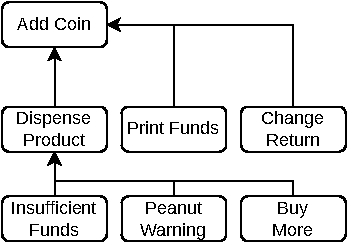
\includegraphics{figures/VendingMachine.pdf}
    \caption{Dependencies between vending machine features.}
    \label{fig:vmDependencies}
\end{figure}

\todo{Base FSM}
\todo{Type Infrastructure}
\todo{Data}

\jnote{I have data for the number of states, tokens, transitions, and LUTs that several different feature combinations create. Do we need the generated lines of verilog too? In past AOP research, I've seen them use (generated lines)/(aspect lines) as an indicator of the efficiency of the aspect code.}

\subsection{Nim}\label{sec:nim}
\subsection{SIMD Cache Coherence}\label{sec:cache}

\section{Future Work}
%%
%% The next two lines define the bibliography style to be used, and
%% the bibliography file.
\bibliographystyle{ACM-Reference-Format}
\bibliography{acmart}

\end{document}
\endinput
%%
%% End of file `sample-sigplan.tex'.
